\documentclass[../TDE3.tex]{subfiles}%

\begin{document}
\section[s]"2"{Circuit RC à 2 mailles}
\noindent

\begin{minipage}{0.50\linewidth}
	On considère le circuit représenté ci-contre, dans lequel l'interrupteur $K$
	est fermé à $t=0$.
\end{minipage}
\hfill
\begin{minipage}{0.45\linewidth}
	\begin{center}
		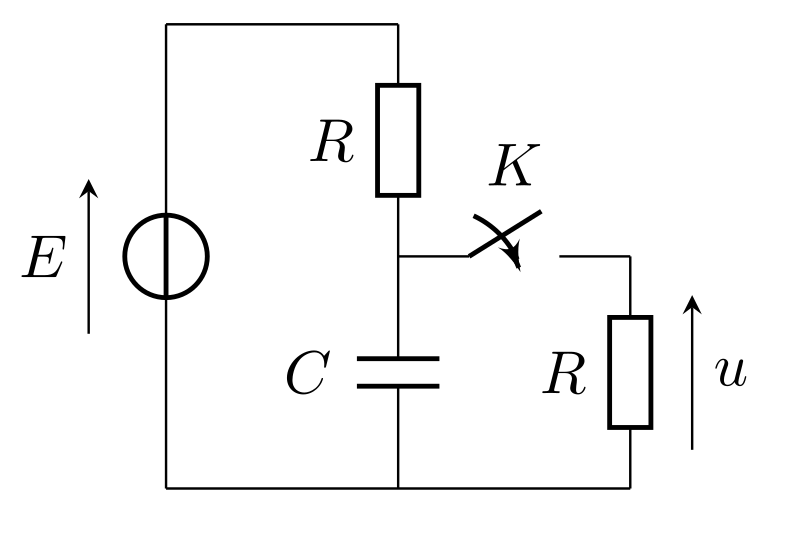
\includegraphics[width=\linewidth]{rc_2mailles-plain}
	\end{center}
\end{minipage}

\QR{%
	Trouver l'expression de la tension $u(t)$ et tracer son allure.
}{%
	LdMailles~:
	\[Ri + u = E \qet u_C = u\]
	LdN~:
	\[i = i_1 + i_2 = C \dv{u_C}{t} + \frac{u}{R}\]
	D'où
	\begin{align*}
		RC \dv{u_C}{t} + 2u           & = E
		\\\Lra
		\dv{u_C}{t} + \frac{1}{\tau}u & = \frac{E}{2\tau}
	\end{align*}
	avec $\tau = \frac{RC}{2}$.
	\smallbreak
	Après résolution avec $u(0^+) = E$, on obtient
	\[ \boxed{u(t) = \frac{E}{2}(1+e^{-t/\tau})}\]
	Ainsi, $u_C$ décroit exponentiellement de $E$ à $E/2$.
}%
\end{document}
